\documentclass[a4paper, 12pt]{article}
%%%%%%%%%%%%%%%%%%%%%%%%%%%%%%%%%%%%%%%%%%%%%%%%%%%%%%%%%%%%%%%%%%%%%%%%%%%%%%%
%                                Basic Packages                               %
%%%%%%%%%%%%%%%%%%%%%%%%%%%%%%%%%%%%%%%%%%%%%%%%%%%%%%%%%%%%%%%%%%%%%%%%%%%%%%%

% Gives us multiple colors.
\usepackage[usenames,dvipsnames,pdftex]{xcolor}
% Lets us style link colors.
\usepackage{hyperref}
% Lets us import images and graphics.
\usepackage{graphicx}
% Lets us use figures in floating environments.
\usepackage{float}
% Lets us create multiple columns.
\usepackage{multicol}
% Gives us better math syntax.
\usepackage{amsmath,amsfonts,mathtools,amsthm,amssymb}
% Lets us strikethrough text.
\usepackage{cancel}
% Lets us edit the caption of a figure.
\usepackage{caption}
% Lets us import pdf directly in our tex code.
\usepackage{pdfpages}
% Lets us do algorithm stuff.
\usepackage[ruled,vlined,linesnumbered]{algorithm2e}
% Use a smiley face for our qed symbol.
\usepackage{tikzsymbols}
% \usepackage{fullpage} %%smaller margins
\usepackage[shortlabels]{enumitem}

\setlist[enumerate]{font={\bfseries}} % global settings, for all lists

\usepackage{setspace}
\usepackage[margin=1in, headsep=12pt]{geometry}
\usepackage{wrapfig}
\usepackage{listings}
\usepackage{parskip}

\definecolor{codegreen}{rgb}{0,0.6,0}
\definecolor{codegray}{rgb}{0.5,0.5,0.5}
\definecolor{codepurple}{rgb}{0.58,0,0.82}
\definecolor{backcolour}{rgb}{0.95,0.95,0.95}

\lstdefinestyle{mystyle}{
    backgroundcolor=\color{backcolour},   
    commentstyle=\color{codegreen},
    keywordstyle=\color{magenta},
    numberstyle=\tiny\color{codegray},
    stringstyle=\color{codepurple},
    basicstyle=\ttfamily\footnotesize,
    breakatwhitespace=false,         
    breaklines=true,                 
    captionpos=b,                    
    keepspaces=true,                 
    numbers=left,                    
    numbersep=5pt,                  
    showspaces=false,                
    showstringspaces=false,
    showtabs=false,                  
    tabsize=2,
    numbers=none
}

\lstset{style=mystyle}
\def\class{article}


%%%%%%%%%%%%%%%%%%%%%%%%%%%%%%%%%%%%%%%%%%%%%%%%%%%%%%%%%%%%%%%%%%%%%%%%%%%%%%%
%                                Basic Settings                               %
%%%%%%%%%%%%%%%%%%%%%%%%%%%%%%%%%%%%%%%%%%%%%%%%%%%%%%%%%%%%%%%%%%%%%%%%%%%%%%%

%%%%%%%%%%%%%
%  Symbols  %
%%%%%%%%%%%%%

\let\implies\Rightarrow
\let\impliedby\Leftarrow
\let\iff\Leftrightarrow
\let\epsilon\varepsilon
%%%%%%%%%%%%
%  Tables  %
%%%%%%%%%%%%

\setlength{\tabcolsep}{5pt}
\renewcommand\arraystretch{1.5}

%%%%%%%%%%%%%%
%  SI Unitx  %
%%%%%%%%%%%%%%

\usepackage{siunitx}
\sisetup{locale = FR}

%%%%%%%%%%
%  TikZ  %
%%%%%%%%%%

\usepackage[framemethod=TikZ]{mdframed}
\usepackage{tikz}
\usepackage{tikz-cd}
\usepackage{tikzsymbols}

\usetikzlibrary{intersections, angles, quotes, calc, positioning}
\usetikzlibrary{arrows.meta}

\tikzset{
    force/.style={thick, {Circle[length=2pt]}-stealth, shorten <=-1pt}
}

%%%%%%%%%%%%%%%
%  PGF Plots  %
%%%%%%%%%%%%%%%

\usepackage{pgfplots}
\pgfplotsset{width=10cm, compat=newest}

%%%%%%%%%%%%%%%%%%%%%%%
%  Center Title Page  %
%%%%%%%%%%%%%%%%%%%%%%%

\usepackage{titling}
\renewcommand\maketitlehooka{\null\mbox{}\vfill}
\renewcommand\maketitlehookd{\vfill\null}

%%%%%%%%%%%%%%%%%%%%%%%%%%%%%%%%%%%%%%%%%%%%%%%%%%%%%%%
%  Create a grey background in the middle of the PDF  %
%%%%%%%%%%%%%%%%%%%%%%%%%%%%%%%%%%%%%%%%%%%%%%%%%%%%%%%

\usepackage{eso-pic}
\newcommand\definegraybackground{
    \definecolor{reallylightgray}{HTML}{FAFAFA}
    \AddToShipoutPicture{
        \ifthenelse{\isodd{\thepage}}{
            \AtPageLowerLeft{
                \put(\LenToUnit{\dimexpr\paperwidth-222pt},0){
                    \color{reallylightgray}\rule{222pt}{297mm}
                }
            }
        }
        {
            \AtPageLowerLeft{
                \color{reallylightgray}\rule{222pt}{297mm}
            }
        }
    }
}

%%%%%%%%%%%%%%%%%%%%%%%%
%  Modify Links Color  %
%%%%%%%%%%%%%%%%%%%%%%%%

\hypersetup{
    % Enable highlighting links.
    colorlinks,
    % Change the color of links to blue.
    urlcolor=blue,
    % Change the color of citations to black.
    citecolor={black},
    % Change the color of url's to blue with some black.
    linkcolor={blue!80!black}
}

%%%%%%%%%%%%%%%%%%
% Fix WrapFigure %
%%%%%%%%%%%%%%%%%%

\newcommand{\wrapfill}{\par\ifnum\value{WF@wrappedlines}>0
        \parskip=0pt
        \addtocounter{WF@wrappedlines}{-1}%
        \null\vspace{\arabic{WF@wrappedlines}\baselineskip}%
        \WFclear
    \fi}

%%%%%%%%%%%%%%%%%
% Multi Columns %
%%%%%%%%%%%%%%%%%

\let\multicolmulticols\multicols
\let\endmulticolmulticols\endmulticols

\RenewDocumentEnvironment{multicols}{mO{}}
{%
    \ifnum#1=1
        #2%
    \else % More than 1 column
        \multicolmulticols{#1}[#2]
    \fi
}
{%
    \ifnum#1=1
    \else % More than 1 column
        \endmulticolmulticols
    \fi
}

\newlength{\thickarrayrulewidth}
\setlength{\thickarrayrulewidth}{5\arrayrulewidth}


%%%%%%%%%%%%%%%%%%%%%%%%%%%%%%%%%%%%%%%%%%%%%%%%%%%%%%%%%%%%%%%%%%%%%%%%%%%%%%%
%                           School Specific Commands                          %
%%%%%%%%%%%%%%%%%%%%%%%%%%%%%%%%%%%%%%%%%%%%%%%%%%%%%%%%%%%%%%%%%%%%%%%%%%%%%%%

%%%%%%%%%%%%%%%%%%%%%%%%%%%
%  Initiate New Counters  %
%%%%%%%%%%%%%%%%%%%%%%%%%%%

\newcounter{lecturecounter}

%%%%%%%%%%%%%%%%%%%%%%%%%%
%  Helpful New Commands  %
%%%%%%%%%%%%%%%%%%%%%%%%%%

\makeatletter

\newcommand\resetcounters{
    % Reset the counters for subsection, subsubsection and the definition
    % all the custom environments.
    \setcounter{subsection}{0}
    \setcounter{subsubsection}{0}
    \setcounter{definition0}{0}
    \setcounter{paragraph}{0}
    \setcounter{theorem}{0}
    \setcounter{claim}{0}
    \setcounter{corollary}{0}
    \setcounter{proposition}{0}
    \setcounter{lemma}{0}
    \setcounter{exercise}{0}
    \setcounter{problem}{0}
    
    \setcounter{subparagraph}{0}
    % \@ifclasswith\class{nocolor}{
    %     \setcounter{definition}{0}
    % }{}
}

%%%%%%%%%%%%%%%%%%%%%
%  Lecture Command  %
%%%%%%%%%%%%%%%%%%%%%

\usepackage{xifthen}

% EXAMPLE:
% 1. \lecture{Oct 17 2022 Mon (08:46:48)}{Lecture Title}
% 2. \lecture[4]{Oct 17 2022 Mon (08:46:48)}{Lecture Title}
% 3. \lecture{Oct 17 2022 Mon (08:46:48)}{}
% 4. \lecture[4]{Oct 17 2022 Mon (08:46:48)}{}
% Parameters:
% 1. (Optional) lecture number.
% 2. Time and date of lecture.
% 3. Lecture Title.
\def\@lecture{}
\def\@lectitle{}
\def\@leccount{}
\newcommand\lecture[3]{
    \newpage

    % Check if user passed the lecture title or not.
    \def\@leccount{Lecture #1}
    \ifthenelse{\isempty{#3}}{
        \def\@lecture{Lecture #1}
        \def\@lectitle{Lecture #1}
    }{
        \def\@lecture{Lecture #1: #3}
        \def\@lectitle{#3}
    }

    \setcounter{section}{#1}
    \renewcommand\thesubsection{#1.\arabic{subsection}}
    
    \phantomsection
    \addcontentsline{toc}{section}{\@lecture}
    \resetcounters

    \begin{mdframed}
        \begin{center}
            \Large \textbf{\@leccount}
            
            \vspace*{0.2cm}
            
            \large \@lectitle
            
            
            \vspace*{0.2cm}

            \normalsize #2
        \end{center}
    \end{mdframed}

}

%%%%%%%%%%%%%%%%%%%%
%  Import Figures  %
%%%%%%%%%%%%%%%%%%%%

\usepackage{import}
\pdfminorversion=7

% EXAMPLE:
% 1. \incfig{limit-graph}
% 2. \incfig[0.4]{limit-graph}
% Parameters:
% 1. The figure name. It should be located in figures/NAME.tex_pdf.
% 2. (Optional) The width of the figure. Example: 0.5, 0.35.
\newcommand\incfig[2][1]{%
    \def\svgwidth{#1\columnwidth}
    \import{./figures/}{#2.pdf_tex}
}

\begingroup\expandafter\expandafter\expandafter\endgroup
\expandafter\ifx\csname pdfsuppresswarningpagegroup\endcsname\relax
\else
    \pdfsuppresswarningpagegroup=1\relax
\fi

%%%%%%%%%%%%%%%%%
% Fancy Headers %
%%%%%%%%%%%%%%%%%

\usepackage{fancyhdr}

% Force a new page.
\newcommand\forcenewpage{\clearpage\mbox{~}\clearpage\newpage}

% This command makes it easier to manage my headers and footers.
\newcommand\createintro{
    % Use roman page numbers (e.g. i, v, vi, x, ...)
    \pagenumbering{roman}

    % Display the page style.
    \maketitle
    % Make the title pagestyle empty, meaning no fancy headers and footers.
    \thispagestyle{empty}
    % Create a newpage.
    \newpage

    % Input the intro.tex page if it exists.
    \IfFileExists{intro.tex}{ % If the intro.tex file exists.
        % Input the intro.tex file.
        \textbf{Course}: MATH 16300: Honors Calculus III

\textbf{Section}: 43

\textbf{Professor}: Minjae Park

\textbf{At}: The University of Chicago

\textbf{Quarter}: Spring 2023

\textbf{Course materials}: Calculus by Spivak (4th Edition), Calculus On Manifolds by Spivak

\vspace{1cm}
\textbf{Disclaimer}: This document will inevitably contain some mistakes, both simple typos and serious logical and mathematical errors. Take what you read with a grain of salt as it is made by an undergraduate student going through the learning process himself. If you do find any error, I would really appreciate it if you can let me know by email at \href{mailto:conghungletran@gmail.com}{conghungletran@gmail.com}.

        % Make the pagestyle fancy for the intro.tex page.
        \pagestyle{fancy}

        % Remove the line for the header.
        \renewcommand\headrulewidth{0pt}

        % Remove all header stuff.
        \fancyhead{}

        % Add stuff for the footer in the center.
        % \fancyfoot[C]{
        %   \textit{For more notes like this, visit
        %   \href{\linktootherpages}{\shortlinkname}}. \\
        %   \vspace{0.1cm}
        %   \hrule
        %   \vspace{0.1cm}
        %   \@author, \\
        %   \term: \academicyear, \\
        %   Last Update: \@date, \\
        %   \faculty
        % }

        \newpage
    }{ % If the intro.tex file doesn't exist.
        % Force a \newpageage.
        % \forcenewpage
        \newpage
    }

    % Remove the center stuff we did above, and replace it with just the page
    % number, which is still in roman numerals.
    \fancyfoot[C]{\thepage}
    % Add the table of contents.
    \tableofcontents
    % Force a new page.
    \newpage

    % Move the page numberings back to arabic, from roman numerals.
    \pagenumbering{arabic}
    % Set the page number to 1.
    \setcounter{page}{1}

    % Add the header line back.
    \renewcommand\headrulewidth{0.4pt}
    % In the top right, add the lecture title.
    \fancyhead[R]{\footnotesize \@lecture}
    % In the top left, add the author name.
    \fancyhead[L]{\footnotesize \@author}
    % In the bottom center, add the page.
    \fancyfoot[C]{\thepage}
    % Add a nice gray background in the middle of all the upcoming pages.
    % \definegraybackground
}

\makeatother


%%%%%%%%%%%%%%%%%%%%%%%%%%%%%%%%%%%%%%%%%%%%%%%%%%%%%%%%%%%%%%%%%%%%%%%%%%%%%%%
%                               Custom Commands                               %
%%%%%%%%%%%%%%%%%%%%%%%%%%%%%%%%%%%%%%%%%%%%%%%%%%%%%%%%%%%%%%%%%%%%%%%%%%%%%%%

%%%%%%%%%%%%
%  Circle  %
%%%%%%%%%%%%

\newcommand*\circled[1]{\tikz[baseline= (char.base)]{
        \node[shape=circle,draw,inner sep=1pt] (char) {#1};}
}

%%%%%%%%%%%%%%%%%%%
%  Todo Commands  %
%%%%%%%%%%%%%%%%%%%

% \usepackage{xargs}
% \usepackage[colorinlistoftodos]{todonotes}

% \makeatletter

% \@ifclasswith\class{working}{
%     \newcommandx\unsure[2][1=]{\todo[linecolor=red,backgroundcolor=red!25,bordercolor=red,#1]{#2}}
%     \newcommandx\change[2][1=]{\todo[linecolor=blue,backgroundcolor=blue!25,bordercolor=blue,#1]{#2}}
%     \newcommandx\info[2][1=]{\todo[linecolor=OliveGreen,backgroundcolor=OliveGreen!25,bordercolor=OliveGreen,#1]{#2}}
%     \newcommandx\improvement[2][1=]{\todo[linecolor=Plum,backgroundcolor=Plum!25,bordercolor=Plum,#1]{#2}}

%     \newcommand\listnotes{
%         \newpage
%         \listoftodos[Notes]
%     }
% }{
%     \newcommandx\unsure[2][1=]{}
%     \newcommandx\change[2][1=]{}
%     \newcommandx\info[2][1=]{}
%     \newcommandx\improvement[2][1=]{}

%     \newcommand\listnotes{}
% }

% \makeatother

%%%%%%%%%%%%%
%  Correct  %
%%%%%%%%%%%%%

% EXAMPLE:
% 1. \correct{INCORRECT}{CORRECT}
% Parameters:
% 1. The incorrect statement.
% 2. The correct statement.
\definecolor{correct}{HTML}{009900}
\newcommand\correct[2]{{\color{red}{#1 }}\ensuremath{\to}{\color{correct}{ #2}}}


%%%%%%%%%%%%%%%%%%%%%%%%%%%%%%%%%%%%%%%%%%%%%%%%%%%%%%%%%%%%%%%%%%%%%%%%%%%%%%%
%                                 Environments                                %
%%%%%%%%%%%%%%%%%%%%%%%%%%%%%%%%%%%%%%%%%%%%%%%%%%%%%%%%%%%%%%%%%%%%%%%%%%%%%%%

\usepackage{varwidth}
\usepackage{thmtools}
\usepackage[most,many,breakable]{tcolorbox}

\tcbuselibrary{theorems,skins,hooks}
\usetikzlibrary{arrows,calc,shadows.blur}

%%%%%%%%%%%%%%%%%%%
%  Define Colors  %
%%%%%%%%%%%%%%%%%%%

% color prototype
% \definecolor{color}{RGB}{45, 111, 177}

% ESSENTIALS: 
\definecolor{myred}{HTML}{c74540}
\definecolor{myblue}{HTML}{072b85}
\definecolor{mygreen}{HTML}{388c46}
\definecolor{myblack}{HTML}{000000}

\colorlet{definition_color}{myred}

\colorlet{theorem_color}{myblue}
\colorlet{lemma_color}{myblue}
\colorlet{prop_color}{myblue}
\colorlet{corollary_color}{myblue}
\colorlet{claim_color}{myblue}

\colorlet{proof_color}{myblack}
\colorlet{example_color}{myblack}
\colorlet{exercise_color}{myblack}

% MISCS: 
%%%%%%%%%%%%%%%%%%%%%%%%%%%%%%%%%%%%%%%%%%%%%%%%%%%%%%%%%
%  Create Environments Styles Based on Given Parameter  %
%%%%%%%%%%%%%%%%%%%%%%%%%%%%%%%%%%%%%%%%%%%%%%%%%%%%%%%%%

% \mdfsetup{skipabove=1em,skipbelow=0em}

%%%%%%%%%%%%%%%%%%%%%%
%  Helpful Commands  %
%%%%%%%%%%%%%%%%%%%%%%

% EXAMPLE:
% 1. \createnewtheoremstyle{thmdefinitionbox}{}{}
% 2. \createnewtheoremstyle{thmtheorembox}{}{}
% 3. \createnewtheoremstyle{thmproofbox}{qed=\qedsymbol}{
%       rightline=false, topline=false, bottomline=false
%    }
% Parameters:
% 1. Theorem name.
% 2. Any extra parameters to pass directly to declaretheoremstyle.
% 3. Any extra parameters to pass directly to mdframed.
\newcommand\createnewtheoremstyle[3]{
    \declaretheoremstyle[
        headfont=\bfseries\sffamily, bodyfont=\normalfont, #2,
        mdframed={
                #3,
            },
    ]{#1}
}

% EXAMPLE:
% 1. \createnewcoloredtheoremstyle{thmdefinitionbox}{definition}{}{}
% 2. \createnewcoloredtheoremstyle{thmexamplebox}{example}{}{
%       rightline=true, leftline=true, topline=true, bottomline=true
%     }
% 3. \createnewcoloredtheoremstyle{thmproofbox}{proof}{qed=\qedsymbol}{backgroundcolor=white}
% Parameters:
% 1. Theorem name.
% 2. Color of theorem.
% 3. Any extra parameters to pass directly to declaretheoremstyle.
% 4. Any extra parameters to pass directly to mdframed.

% change backgroundcolor to #2!5 if user wants a colored backdrop to theorem environments. It's a cool color theme, but there's too much going on in the page.
\newcommand\createnewcoloredtheoremstyle[4]{
    \declaretheoremstyle[
        headfont=\bfseries\sffamily\color{#2},
        bodyfont=\normalfont,
        headpunct=,
        headformat = \NAME~\NUMBER\NOTE \hfill\smallskip\linebreak,
        #3,
        mdframed={
                outerlinewidth=0.75pt,
                rightline=false,
                leftline=false,
                topline=false,
                bottomline=false,
                backgroundcolor=white,
                skipabove = 5pt,
                skipbelow = 0pt,
                linecolor=#2,
                innertopmargin = 0pt,
                innerbottommargin = 0pt,
                innerrightmargin = 4pt,
                innerleftmargin= 6pt,
                leftmargin = -6pt,
                #4,
            },
    ]{#1}
}



%%%%%%%%%%%%%%%%%%%%%%%%%%%%%%%%%%%
%  Create the Environment Styles  %
%%%%%%%%%%%%%%%%%%%%%%%%%%%%%%%%%%%

\makeatletter
\@ifclasswith\class{nocolor}{
    % Environments without color.

    % ESSENTIALS:
    \createnewtheoremstyle{thmdefinitionbox}{}{}
    \createnewtheoremstyle{thmtheorembox}{}{}
    \createnewtheoremstyle{thmproofbox}{qed=\qedsymbol}{}
    \createnewtheoremstyle{thmcorollarybox}{}{}
    \createnewtheoremstyle{thmlemmabox}{}{}
    \createnewtheoremstyle{thmclaimbox}{}{}
    \createnewtheoremstyle{thmexamplebox}{}{}

    % MISCS: 
    \createnewtheoremstyle{thmpropbox}{}{}
    \createnewtheoremstyle{thmexercisebox}{}{}
    \createnewtheoremstyle{thmexplanationbox}{}{}
    \createnewtheoremstyle{thmremarkbox}{}{}
    
    % STYLIZED MORE BELOW
    \createnewtheoremstyle{thmquestionbox}{}{}
    \createnewtheoremstyle{thmsolutionbox}{qed=\qedsymbol}{}
}{
    % Environments with color.

    % ESSENTIALS: definition, theorem, proof, corollary, lemma, claim, example
    \createnewcoloredtheoremstyle{thmdefinitionbox}{definition_color}{}{leftline=false}
    \createnewcoloredtheoremstyle{thmtheorembox}{theorem_color}{}{leftline=false}
    \createnewcoloredtheoremstyle{thmproofbox}{proof_color}{qed=\qedsymbol}{}
    \createnewcoloredtheoremstyle{thmcorollarybox}{corollary_color}{}{leftline=false}
    \createnewcoloredtheoremstyle{thmlemmabox}{lemma_color}{}{leftline=false}
    \createnewcoloredtheoremstyle{thmpropbox}{prop_color}{}{leftline=false}
    \createnewcoloredtheoremstyle{thmclaimbox}{claim_color}{}{leftline=false}
    \createnewcoloredtheoremstyle{thmexamplebox}{example_color}{}{}
    \createnewcoloredtheoremstyle{thmexplanationbox}{example_color}{qed=\qedsymbol}{}
    \createnewcoloredtheoremstyle{thmremarkbox}{theorem_color}{}{}

    \createnewcoloredtheoremstyle{thmmiscbox}{black}{}{}

    \createnewcoloredtheoremstyle{thmexercisebox}{exercise_color}{}{}
    \createnewcoloredtheoremstyle{thmproblembox}{theorem_color}{}{leftline=false}
    \createnewcoloredtheoremstyle{thmsolutionbox}{mygreen}{qed=\qedsymbol}{}
}
\makeatother

%%%%%%%%%%%%%%%%%%%%%%%%%%%%%
%  Create the Environments  %
%%%%%%%%%%%%%%%%%%%%%%%%%%%%%
\declaretheorem[numberwithin=section, style=thmdefinitionbox,     name=Definition]{definition}
\declaretheorem[numberwithin=section, style=thmtheorembox,     name=Theorem]{theorem}
\declaretheorem[numbered=no,          style=thmexamplebox,     name=Example]{example}
\declaretheorem[numberwithin=section, style=thmtheorembox,       name=Claim]{claim}
\declaretheorem[numberwithin=section, style=thmcorollarybox,   name=Corollary]{corollary}
\declaretheorem[numberwithin=section, style=thmpropbox,        name=Proposition]{proposition}
\declaretheorem[numberwithin=section, style=thmlemmabox,       name=Lemma]{lemma}
\declaretheorem[numberwithin=section, style=thmexercisebox,    name=Exercise]{exercise}
\declaretheorem[numbered=no,          style=thmproofbox,       name=Proof]{proof0}
\declaretheorem[numbered=no,          style=thmexplanationbox, name=Explanation]{explanation}
\declaretheorem[numbered=no,          style=thmsolutionbox,    name=Solution]{solution}
\declaretheorem[numberwithin=section,          style=thmproblembox,     name=Problem]{problem}
\declaretheorem[numbered=no,          style=thmmiscbox,    name=Intuition]{intuition}
\declaretheorem[numbered=no,          style=thmmiscbox,    name=Goal]{goal}
\declaretheorem[numbered=no,          style=thmmiscbox,    name=Recall]{recall}
\declaretheorem[numbered=no,          style=thmmiscbox,    name=Motivation]{motivation}
\declaretheorem[numbered=no,          style=thmmiscbox,    name=Remark]{remark}
\declaretheorem[numbered=no,          style=thmmiscbox,    name=Observe]{observe}
\declaretheorem[numbered=no,          style=thmmiscbox,    name=Question]{question}


%%%%%%%%%%%%%%%%%%%%%%%%%%%%
%  Edit Proof Environment  %
%%%%%%%%%%%%%%%%%%%%%%%%%%%%

\renewenvironment{proof}[2][\proofname]{
    % \vspace{-12pt}
    \begin{proof0} [#2]
        }{\end{proof0}}

\theoremstyle{definition}

\newtheorem*{notation}{Notation}
\newtheorem*{previouslyseen}{As previously seen}
\newtheorem*{property}{Property}
% \newtheorem*{intuition}{Intuition}
% \newtheorem*{goal}{Goal}
% \newtheorem*{recall}{Recall}
% \newtheorem*{motivation}{Motivation}
% \newtheorem*{remark}{Remark}
% \newtheorem*{observe}{Observe}

\author{Hung C. Le Tran}


%%%% MATH SHORTHANDS %%%%
%% blackboard bold math capitals
\DeclareMathOperator*{\esssup}{ess\,sup}
\DeclareMathOperator*{\Hom}{Hom}
\newcommand{\bbf}{\mathbb{F}}
\newcommand{\bbn}{\mathbb{N}}
\newcommand{\bbq}{\mathbb{Q}}
\newcommand{\bbr}{\mathbb{R}}
\newcommand{\bbz}{\mathbb{Z}}
\newcommand{\bbc}{\mathbb{C}}
\newcommand{\bbk}{\mathbb{K}}
\newcommand{\bbm}{\mathbb{M}}
\newcommand{\bbp}{\mathbb{P}}
\newcommand{\bbe}{\mathbb{E}}

\newcommand{\bfw}{\mathbf{w}}
\newcommand{\bfx}{\mathbf{x}}
\newcommand{\bfX}{\mathbf{X}}
\newcommand{\bfy}{\mathbf{y}}
\newcommand{\bfyhat}{\mathbf{\hat{y}}}

\newcommand{\calb}{\mathcal{B}}
\newcommand{\calf}{\mathcal{F}}
\newcommand{\calt}{\mathcal{T}}
\newcommand{\call}{\mathcal{L}}
\renewcommand{\phi}{\varphi}

% Universal Math Shortcuts
\newcommand{\st}{\hspace*{2pt}\text{s.t.}\hspace*{2pt}}
\newcommand{\pffwd}{\hspace*{2pt}\fbox{\(\Rightarrow\)}\hspace*{10pt}}
\newcommand{\pfbwd}{\hspace*{2pt}\fbox{\(\Leftarrow\)}\hspace*{10pt}}
\newcommand{\contra}{\ensuremath{\Rightarrow\Leftarrow}}
\newcommand{\cvgn}{\xrightarrow{n \to \infty}}
\newcommand{\cvgj}{\xrightarrow{j \to \infty}}

\newcommand{\im}{\mathrm{im}}
\newcommand{\innerproduct}[2]{\langle #1, #2 \rangle}
\newcommand*{\conj}[1]{\overline{#1}}

% https://tex.stackexchange.com/questions/438612/space-between-exists-and-forall
% https://tex.stackexchange.com/questions/22798/nice-looking-empty-set
\let\oldforall\forall
\renewcommand{\forall}{\;\oldforall\; }
\let\oldexist\exists
\renewcommand{\exists}{\;\oldexist\; }
\newcommand\existu{\;\oldexist!\: }
\let\oldemptyset\emptyset
\let\emptyset\varnothing


\renewcommand{\_}[1]{\underline{#1}}
\DeclarePairedDelimiter{\abs}{\lvert}{\rvert}
\DeclarePairedDelimiter{\norm}{\lVert}{\rVert}
\DeclarePairedDelimiter\ceil{\lceil}{\rceil}
\DeclarePairedDelimiter\floor{\lfloor}{\rfloor}
\setlength\parindent{0pt}
\setlength{\headheight}{12.0pt}
\addtolength{\topmargin}{-12.0pt}


% Default skipping, change if you want more spacing
% \thinmuskip=3mu
% \medmuskip=4mu plus 2mu minus 4mu
% \thickmuskip=5mu plus 5mu

% \DeclareMathOperator{\ext}{ext}
% \DeclareMathOperator{\bridge}{bridge}
\title{CMSC 25300: Mathematical Foundations of ML \\ \large Problem Set 3}
\date{21 Oct 2023}
\author{Hung Le Tran}
\begin{document}
\maketitle
\setcounter{section}{3}
\begin{problem} [Problem 1]
\end{problem}
\begin{solution}
    (a) $\bfX_1 = \begin{bmatrix}
            3 \\ 0 \\ 0
        \end{bmatrix} \bfX_2 = \begin{bmatrix}
            1 \\ 3 \\ 3
        \end{bmatrix}$. Gram-Schimdt:
    \[
        \bfU_1 = \frac{\bfX_1}{||\bfX_1||} = \frac{1}{3}\begin{bmatrix}
            3 \\ 0 \\ 0
        \end{bmatrix} = \begin{bmatrix}
            1 \\ 0 \\ 0
        \end{bmatrix}
    \]
    \[
        \bfX_2' = \bfX_2 - \bfU_1 (\bfU_1^T \bfX_2) = \begin{bmatrix}
            1 \\ 3 \\ 3
        \end{bmatrix} - 1\begin{bmatrix}
            1 \\ 0 \\ 0
        \end{bmatrix} = \begin{bmatrix}
            0 \\ 3 \\ 3
        \end{bmatrix}
    \]
    \[
        \implies \bfU_2 = \frac{1}{\sqrt{18}}\begin{bmatrix}
            0 \\ 3 \\ 3
        \end{bmatrix} = \begin{bmatrix}
            0 \\ 1/\sqrt{2} \\ 1/\sqrt{2}
        \end{bmatrix}
    \]

    (b)
    \[
        \bfU = \begin{bmatrix}
            1 & 0          \\
            0 & 1/\sqrt{2} \\
            0 & 1/\sqrt{2}
        \end{bmatrix}
    \]

    The LS estimate $\bfyhat$ is nothing more than the point on the subspace $S$ spanned by the columns of $\bfX$ that is closest to $\bfy$, i.e. the projection of $\bfyhat$ on $S$. This is \[
        \bfyhat = \bfX(\bfX^T \bfX)^{-1} \bfX^T \bfy
    \]
    However, this space $S$ also spanned by the columns of $\bfU$, as it is simply the orthogonalization of the columns of $\bfX$. It follows that one can also retrieve the LS-estimate:\[
        \bfyhat = \bfU(\bfU^T \bfU)^{-1} \bfU^T \bfy
    \]

    (c) Computing the LS-estimate is easier using $\bfU$ because \[
        \bfU^T \bfU = 1
    \]
    so the estimate is simply \[
        \bfyhat = \bfU(\bfU^T \bfy)
    \]
    In this example, \begin{align*}
        \bfyhat & = \bfU \left(\begin{bmatrix}
                                   1 & 0          & 0          \\
                                   0 & 1/\sqrt{2} & 1/\sqrt{2}
                               \end{bmatrix} \begin{bmatrix}
                                                 1 \\ 6 \\ -2
                                             \end{bmatrix}\right) \\
                & = \bfU \begin{bmatrix}
                             1 \\
                             2\sqrt{2}
                         \end{bmatrix}                           \\
                & = \begin{bmatrix}
                        1 & 0          \\
                        0 & 1/\sqrt{2} \\
                        0 & 1/\sqrt{2}
                    \end{bmatrix} \begin{bmatrix}
                                      1 \\
                                      2\sqrt{2}
                                  \end{bmatrix} = \begin{bmatrix}
                                                      1 \\
                                                      2 \\
                                                      2
                                                  \end{bmatrix}
    \end{align*}
\end{solution}

\begin{problem} [Problem 2]
\end{problem}
\begin{solution}
    (a)
    \[
        S = \{\bfx \in \bbr^3 \mid 4x_1 - x_2 - 2x_3 = 0\}
    \]
    If $(x_1, x_2, x_3) \in S$ then if $x_3 = 2t, x_2 = 4s$ then $x_1 = t + s$. It follows that \[
        S = \{\bfx \in \bbr^3 \mid x_1 = t + s, x_2 = 4s, x_3 = 2t \:\text{for some}\: t, s \in \bbr\}
    \]
    It follows that any $\bfx \in S$ can be represented as \[
        \begin{bmatrix}
            t + s \\
            4s    \\
            2t
        \end{bmatrix} =     t \begin{bmatrix}
            1 \\ 0 \\ 2
        \end{bmatrix} + s \begin{bmatrix}
            1 \\ 4 \\ 0
        \end{bmatrix}
    \]
    We have found a non-orthonormal basis of $S$: \[
        \bfX = \begin{bmatrix}
            1 & 1 \\
            0 & 4 \\
            2 & 0
        \end{bmatrix}
    \]
    And the corresponding projection matrix is
    \begin{align*}
        \bfP & = \bfX(\bfX^T \bfX)^{-1}\bfX^T \\
             & = \begin{bmatrix}
                     1 & 1 \\
                     0 & 4 \\
                     2 & 0
                 \end{bmatrix}
        \left(\begin{bmatrix}
                  1 & 0 & 2 \\
                  1 & 4 & 0
              \end{bmatrix}
        \begin{bmatrix}
            1 & 1 \\
            0 & 4 \\
            2 & 0
        \end{bmatrix}
        \right)^{-1}
        \begin{bmatrix}
            1 & 0 & 2 \\
            1 & 4 & 0
        \end{bmatrix}  \\
             & =\begin{bmatrix}
                1 & 1 \\
                0 & 4 \\
                2 & 0
            \end{bmatrix}
            \left(
                \begin{bmatrix}
                5 & 1 \\
                1 & 17
                \end{bmatrix}
            \right)^{-1}
            \begin{bmatrix}
                1 & 0 & 2 \\
                1 & 4 & 0
            \end{bmatrix}  \\
            &= \frac{1}{84}\begin{bmatrix}
                1 & 1 \\
                0 & 4 \\
                2 & 0
            \end{bmatrix}
            \begin{bmatrix}
                17 & -1 \\
                -1 & 5
            \end{bmatrix}
            \begin{bmatrix}
                1 & 0 & 2 \\
                1 & 4 & 0
            \end{bmatrix} \\
            &= \frac{1}{21}\begin{bmatrix}
            5 & 4 & 8 \\
            4 & 20 & -2 \\
            8 & -2 & 17
            \end{bmatrix}
    \end{align*}

    (b) Gram-Schmidt: \[
    \bfU_1 = \frac{\bfX_1}{||\bfX_1||} = \begin{bmatrix}
    1 / \sqrt{5} \\
    0\\
    2/\sqrt{5}
    \end{bmatrix}
    \]
    \[
    \bfX_2' = \bfX_2 - \bfU_1(\bfU_1^T\bfX_2) = \begin{bmatrix}
    1 \\ 4 \\ 0
    \end{bmatrix} - \begin{bmatrix}
        1 / \sqrt{5} \\
        0\\
        2/\sqrt{5}
        \end{bmatrix}
        \left(\begin{bmatrix}
        1/\sqrt{5} & 0 & 2/\sqrt{5}
        \end{bmatrix}\begin{bmatrix}
        1 \\ 4 \\ 0
        \end{bmatrix}\right) = \begin{bmatrix}
        4/5 \\ 4 \\ -2/5
        \end{bmatrix}
    \]
    So \[
    \bfU_2 = \sqrt{\frac{5}{84}}\begin{bmatrix}
        4/5 \\ 4 \\ -2/5
        \end{bmatrix} =
        \begin{bmatrix}
        4/\sqrt{420} \\
        20/\sqrt{420}\\
        -2/\sqrt{420}
        \end{bmatrix} = \begin{bmatrix}
        2/\sqrt{105} \\
        10/\sqrt{105} \\
        -1/\sqrt{105}
        \end{bmatrix}
    \]
        The projection matrix is therefore \[
        \bfU\bfU^T = \begin{bmatrix}
        1/\sqrt{5} & 2/\sqrt{105} \\
        0 & 10\sqrt{105} \\
        2/\sqrt{5} & -1/\sqrt{105}
        \end{bmatrix}
        \begin{bmatrix}
        1/\sqrt{5} & 0 & 2/\sqrt{5}\\
        2/\sqrt{105} & 10/\sqrt{105} & -1/\sqrt{105}
        \end{bmatrix}
        = \frac{1}{21}\begin{bmatrix}
            5 & 4 & 8 \\
            4 & 20 & -2 \\
            8 & -2 & 17
            \end{bmatrix}
        \]

        (c)
        \[
        \bfyhat_1 = \frac{1}{21}\begin{bmatrix}
            5 & 4 & 8 \\
            4 & 20 & -2 \\
            8 & -2 & 17
            \end{bmatrix}\begin{bmatrix}
            1 \\
            0 \\
            0
            \end{bmatrix} =
            \frac{1}{21}
            \begin{bmatrix}
                5\\4\\8
            \end{bmatrix}
        \]
        \[
        \bfyhat_2 = \frac{1}{21}\begin{bmatrix}
            5 & 4 & 8 \\
            4 & 20 & -2 \\
            8 & -2 & 17
            \end{bmatrix}\begin{bmatrix}
            1 \\2\\1
            \end{bmatrix} = \frac{1}{21}\begin{bmatrix}
            21 \\
            42 \\
            21
            \end{bmatrix} = \begin{bmatrix}
            1\\
            2\\
            1
            \end{bmatrix}
        \]
        So the distance from $\bfx_1$ is $d(\begin{bmatrix}
            1 \\ 0 \\ 0
        \end{bmatrix}, \begin{bmatrix}
            5/21 \\ 4/21 \\ 8/21
        \end{bmatrix}) = \sqrt{16/21} = 4/\sqrt{21}$
        
        The distance from $\bfx_2$ is $d(\begin{bmatrix}
        1 \\ 2 \\ 1
        \end{bmatrix}, \begin{bmatrix}
        1 \\ 2 \\ 1
        \end{bmatrix}) = 0$
\end{solution}

\begin{problem} [Problem 3]
\end{problem}
\begin{solution}

(a)
Carry out mini-classification problems for each type of iris. e.g. The first mini-classification classifies if the iris is setosa or not. In this mini-classification, assign $\bfy = 1$ if setosa, $-1$ otherwise. Perform this across all $\bfX$, then choose the label with the highest $\bfyhat$ as the final label.

(b) For each mini-classification problem:
\begin{lstlisting} [language=python]
import numpy as np
import scipy.io
import matplotlib.pyplot as plt
from matplotlib import colors
# load data, make sure 'fisheriris.mat' is in your working directory
data = scipy.io.loadmat("fisheriris.mat")
X = data['meas']
y_text = data['species']
############################
# YOUR CODE BELOW
# Process and assign numerical values to
# 'y' according to your (a), make sure 'y' is a 1d numpy array.
TYPES = ['setosa', 'versicolor', 'virginica']
# If dimensions are mismatching, you may find 'y = y.flatten()' useful.
# Compute the least squares weights
for type_index, type in enumerate(TYPES):
    y = y_text == type
    w = np.linalg.inv(X.T @ X) @ X.T @ y
    # Compute the residuals
    r = y - X @ w
    # Make a plot
    print((X@w).T @ r)
    \end{lstlisting}
prints
\begin{lstlisting}
[[-1.97915772e-13]]
[[-3.9014575e-13]]
[[-7.70567792e-13]]
\end{lstlisting}
which is essentially 0.

(c)
\begin{lstlisting} [language=python]
# STARTER CODE
import numpy as np
import scipy.io
# load data, make sure 'fisheriris.mat' is in your working directory
data = scipy.io.loadmat("fisheriris.mat")
# training data
X = data['meas']
y_text = data['species']
y_numberized = (y_text == 'versicolor').astype(int) + (y_text == 'virginica').astype(int)*2
# maps setosa to 0, versicolor to 1, virginica to 2
TYPES = ['setosa', 'versicolor', 'virginica']
# number of random trials
N = 10000
# array to store errors
errs = np.zeros(N)
# size of training set
num_train = 40
for i in np.arange(N):
# initialize 0-length arrays for the train and holdout indices. These
# arrays will be filled in the inner loop.
    idx_train = np.zeros(0, dtype=np.intp)
    idx_holdout = np.zeros(0, dtype=np.intp)

    # There are 3 label types and 50 samples of each type
    for label_type in range(3):
        # Choose a random ordering of the 50 samples
        r = np.random.permutation(50)
        # Add the first num_train indices of the random ordering to
        # the idx_train array
        idx_train = np.concatenate((idx_train,
        50 * label_type + r[:num_train]))
        # Add the rest of the indices to the idx_holdout array
        idx_holdout = np.concatenate((idx_holdout,
        50 * label_type + r[num_train:]))
        # divide data and labels into the train and holdout sets
    
    yhattypes = list()
    for type_index, type in enumerate(TYPES):
        y = (y_text == type).astype(int)
        Xt = X[idx_train]
        yt = y[idx_train]
        Xh = X[idx_holdout]
        yh = y[idx_holdout]
        w = np.linalg.inv(Xt.T @ Xt) @ Xt.T @ yt
        # Make predictions using the LS weights
        yhat = Xh @ w
        yhattypes.append(yhat)
    
    yhattypes = np.array(yhattypes)
    # gives best prediction
    y_pred_numberized = np.argmax(yhattypes, axis = 0)
    # # Turn the real-valued predictions into class labels
    # # Compute the errors
    errs[i] = np.sum(y_pred_numberized != y_numberized[idx_holdout])/30

print(np.average(errs))
\end{lstlisting}
which prints out
\begin{lstlisting}
0.18694666666666668
\end{lstlisting}

(d)
\begin{lstlisting} [language=python]
# STARTER CODE
import numpy as np
import scipy.io
import matplotlib.pyplot as plt
# load data, make sure 'fisheriris.mat' is in your working directory
data = scipy.io.loadmat("fisheriris.mat")
# training data
X = data['meas']
y_text = data['species']
y_numberized = (y_text == 'versicolor').astype(int) + (y_text == 'virginica').astype(int)*2
# maps setosa to 0, versicolor to 1, virginica to 2
TYPES = ['setosa', 'versicolor', 'virginica']
N = 1000
# Min / Max size of the training set
min_num_train = 4
max_num_train = 40
# Arrays to store error rates
train_errs = np.zeros((max_num_train-min_num_train, N))
test_errs = np.zeros((max_num_train-min_num_train, N))
n_train_vals = np.arange(min_num_train, max_num_train)
for j, n_train in enumerate(n_train_vals):
    for i in np.arange(N):
        # initialize 0-length arrays for the train and holdout indices. These
        # arrays will be filled in the inner loop.
        idx_train = np.zeros(0, dtype=np.intp)
        idx_holdout = np.zeros(0, dtype=np.intp)

        # There are 3 label types and 50 samples of each type
        for label_type in range(3):
            # Choose a random ordering of the 50 samples
            r = np.random.permutation(50)
            # Add the first num_train indices of the random ordering to
            # the idx_train array
            idx_train = np.concatenate((idx_train,
            50 * label_type + r[:num_train]))
            # Add the rest of the indices to the idx_holdout array
            idx_holdout = np.concatenate((idx_holdout,
            50 * label_type + r[num_train:]))
            # divide data and labels into the train and holdout sets
        
        yhat_h_all = list()
        yhat_t_all = list()
        for type_index, type in enumerate(TYPES):
            y = (y_text == type).astype(int)
            Xt = X[idx_train]
            yt = y[idx_train]
            Xh = X[idx_holdout]
            yh = y[idx_holdout]
            w = np.linalg.inv(Xt.T @ Xt) @ Xt.T @ yt
            # Make predictions using the LS weights
            yhat_t = Xt @ w
            yhat_h = Xh @ w
            
            yhat_t_all.append(yhat_t)
            yhat_h_all.append(yhat_h)
        
        yhat_t_all = np.array(yhat_t_all)
        yhat_h_all = np.array(yhat_h_all)
        # gives best prediction
        yhat_t_numberized = np.argmax(yhat_t_all, axis = 0)
        yhat_h_numberized = np.argmax(yhat_h_all, axis = 0)
        # # Turn the real-valued predictions into class labels
        # # Compute the errors
        
        train_errs[j][i] = np.sum(yhat_t_numberized != y_numberized[idx_train])/len(yhat_t_numberized)
        test_errs[j][i] = np.sum(yhat_h_numberized != y_numberized[idx_holdout])/len(yhat_h_numberized)

# Make a plot of the train and test errors as a function of
# training set size
yplot_train = np.mean(train_errs, axis = 1)
yplot_test = np.mean(test_errs, axis = 1)

plt.plot(n_train_vals, yplot_train, color='red')
plt.plot(n_train_vals, yplot_test, color='blue')
\end{lstlisting} 
which plots 
\begin{center}
    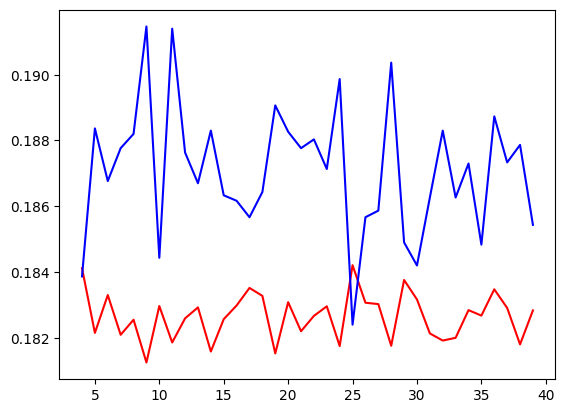
\includegraphics[width=8cm]{./figures/3.3.png}
\end{center}
The trend of test set accuracy and train set error rates seem to be in opposite directions. When train set error rate decreases (fitting better to train set), error rate for test set increases (fitting worse to test set, generalizing worse). The balance between test set and train set error rates seems to be at train set size of 25.


(e)
Use training set size as 25.
\begin{lstlisting} [language=python]
# STARTER CODE
import numpy as np
import scipy.io
# load data, make sure 'fisheriris.mat' is in your working directory
data = scipy.io.loadmat("fisheriris.mat")
# training data
X = data['meas']
# only choosing 1st and 3rd column of X`'
X = X[:, [0, 2]]
y_text = data['species']
y_numberized = (y_text == 'versicolor').astype(int) + (y_text == 'virginica').astype(int)*2
# maps setosa to 0, versicolor to 1, virginica to 2
TYPES = ['setosa', 'versicolor', 'virginica']
# number of random trials
N = 10000
# array to store errors
errs = np.zeros(N)
# size of training set
num_train = 25
for i in np.arange(N):
    # initialize 0-length arrays for the train and holdout indices. These
    # arrays will be filled in the inner loop.
    idx_train = np.zeros(0, dtype=np.intp)
    idx_holdout = np.zeros(0, dtype=np.intp)

    # There are 3 label types and 50 samples of each type
    for label_type in range(3):
        # Choose a random ordering of the 50 samples
        r = np.random.permutation(50)
        # Add the first num_train indices of the random ordering to
        # the idx_train array
        idx_train = np.concatenate((idx_train,
        50 * label_type + r[:num_train]))
        # Add the rest of the indices to the idx_holdout array
        idx_holdout = np.concatenate((idx_holdout,
        50 * label_type + r[num_train:]))
        # divide data and labels into the train and holdout sets
    
    yhat_h_all = list()
    yhat_t_all = list()
    for type_index, type in enumerate(TYPES):
        y = (y_text == type).astype(int)
        Xt = X[idx_train]
        yt = y[idx_train]
        Xh = X[idx_holdout]
        yh = y[idx_holdout]
        w = np.linalg.inv(Xt.T @ Xt) @ Xt.T @ yt
        # Make predictions using the LS weights
        yhat_t = Xt @ w
        yhat_h = Xh @ w
        
        yhat_t_all.append(yhat_t)
        yhat_h_all.append(yhat_h)
    
    yhat_t_all = np.array(yhat_t_all)
    yhat_h_all = np.array(yhat_h_all)
    # gives best prediction
    yhat_t_numberized = np.argmax(yhat_t_all, axis = 0)
    yhat_h_numberized = np.argmax(yhat_h_all, axis = 0)
    # # Turn the real-valued predictions into class labels
    # # Compute the errors
    errs[i] = np.sum(yhat_h_numberized != y_numberized[idx_holdout])/30

print(np.average(errs))
\end{lstlisting}
which prints out
\begin{lstlisting} [language=python]
0.8332233333333335
\end{lstlisting}
Accuracy is drastically reduced when only using 2 out of 4 available features.
\end{solution}

\begin{problem} [Problem 4]
\end{problem}
\begin{solution}
(a) Projecting some points in $\bbr^3$ onto $S$,  
\[
P_S \begin{bmatrix}
1 \\ 0 \\ 0
\end{bmatrix} = \begin{bmatrix}
0.2 \\
0.4 \\
0
\end{bmatrix}
\]
\[
P_S \begin{bmatrix}
0 \\ 0 \\ 1
\end{bmatrix} = \begin{bmatrix}
    0 \\ 0 \\ 1
\end{bmatrix}
\]
And the 2 projected points are linearly independent. Since $Rank(P_S) = 2$, they span the entire subspace $S$. We've found a basis \[
\bfX = \begin{bmatrix}
0.2 & 0 \\
0.4& 0 \\
0 & 1
\end{bmatrix}
\]

(b)
We can take the residual from $\begin{bmatrix}
    0  \\ 1 \\ 0
\end{bmatrix}$. Projecting it to $S$, we have \[
P_S \begin{bmatrix}
0 \\ 1 \\ 0
\end{bmatrix} = \begin{bmatrix}
0.4 \\
0.8 \\
0
\end{bmatrix}
\]
which yields residual $\begin{bmatrix}
-0.4 \\
0.2 \\
0
\end{bmatrix}$.

Since the point lies on $S$, they have to satisfy \[
\begin{bmatrix}
-0.4 & 0.2 & 0
\end{bmatrix}
\begin{bmatrix}
x_1 \\ x_2 \\ x_3
\end{bmatrix} = 0
\]
It follows that \[
-0.4x_1 + 0.2x_2 + 0x_3 = 0
\]

(c)
\begin{lstlisting} [language=python]
### STARTER CODE
import numpy as np
import numpy.linalg as la
import scipy
p = np.array(
[[0.2, 0.4, 0. ],
[0.4, 0.8, 0. ],
[0. , 0. , 1. ]]
)
### YOUR CODE BELOW
print(scipy.linalg.orth(p))
\end{lstlisting}
\end{solution}
\end{document}